\documentclass[11pt]{article}
\usepackage{amsmath, amssymb, amsthm}
\usepackage{geometry}
\usepackage{graphicx}
\usepackage{subcaption} % make sure this is here
\geometry{margin=1in}
\setlength\parindent{0pt}
\title{Foundations of Machine Learning -- Lecture 6 Notes}
\author{}
\date{}

\begin{document}
\maketitle

\section*{Clustering}

Dimensionality Reduction
\[
	X \in \mathbb{R}^{Nxd} \rightarrow Z \in \mathbb{R}^{Nxm}, m << d
\]

Clustering
\[
	X \in \mathbb{R}^{Nxd} \rightarrow Z \in \mathbb{R}^{kxd}, k << N
\]

The main idea with clustering is to reduce the number of data points within a particular set by grouping together similar instances.

\begin{figure}[h]
	\centering
	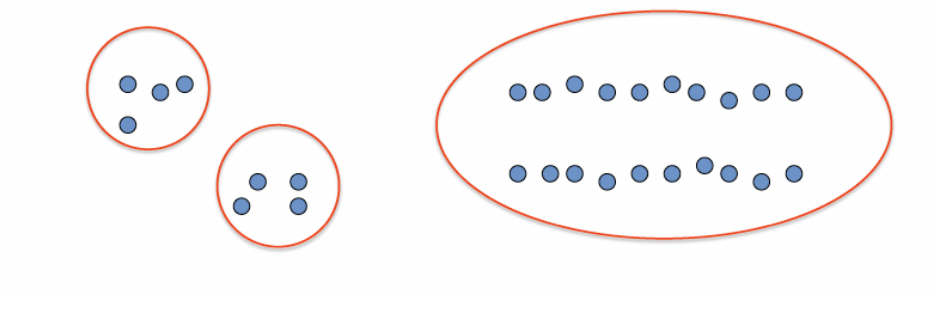
\includegraphics[width=0.35\textwidth]{../imgs/clust-exam.png} % 
\end{figure}

To find out weather points are similar we use a distance formula.
\[
	dist(x^{(i)}, x^{(j)})
\]

\section*{K-Means Clustering}

This is an iterative algorithm for clustering
\medskip

Input: Data ${x^{(i)},\dots,x^{(N)} \in \mathbb{R}^d}$
\medskip

Output: Centroids ${u^{(i)},\dots,x^{(K)} \in \mathbb{R}^d}$
\medskip

Process:
\begin{enumerate}
	\item Initilaize with K random centroids
	\item Repeat until convergence
	      \begin{itemize}
		      \item Assign a cluster to every sample $x^{(i)} \Rightarrow c^{(i)} = \arg\min_k dist(x^{(i)}, u^{(k)})$
		      \item Update centroids according to clusters: \[
			            \mu^{(k)} =
			            \frac{\displaystyle \sum_{i=1}^{N} \mathbf{1}_{c_i = k} \, x^{(i)}}
			            {\displaystyle \sum_{i=1}^{N} \mathbf{1}_{c_i = k}}
		            \]

	      \end{itemize}
\end{enumerate}

\pagebreak

\begin{figure}[h]
	\centering
	\begin{subfigure}[b]{0.24\textwidth}
		\centering
		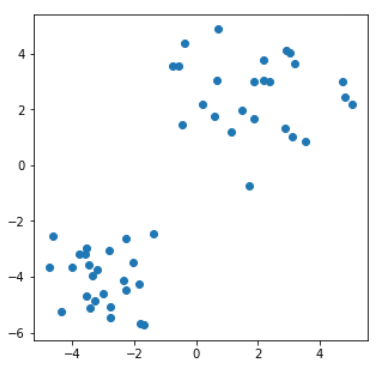
\includegraphics[width=\linewidth]{../imgs/knn-proc-1.png}
		\caption{Step 1}
	\end{subfigure}
	\begin{subfigure}[b]{0.24\textwidth}
		\centering
		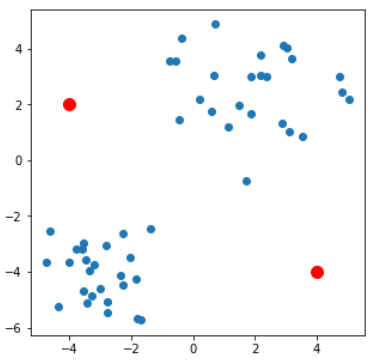
\includegraphics[width=\linewidth]{../imgs/knn-proc-2.png}
		\caption{Step 2}
	\end{subfigure}
	\begin{subfigure}[b]{0.24\textwidth}
		\centering
		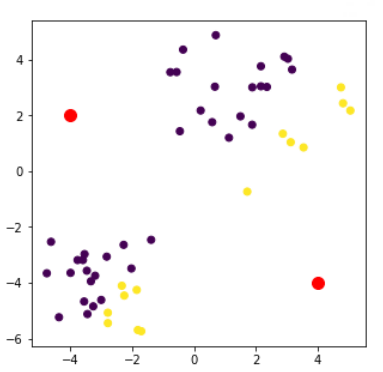
\includegraphics[width=\linewidth]{../imgs/knn-proc-3.png}
		\caption{Step 3}
	\end{subfigure}
	\begin{subfigure}[b]{0.24\textwidth}
		\centering
		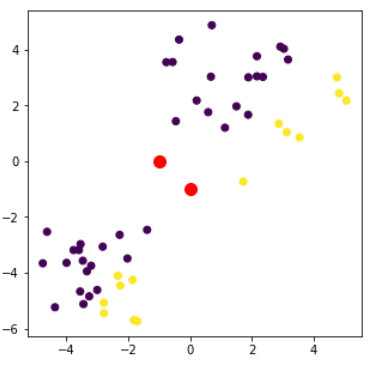
\includegraphics[width=\linewidth]{../imgs/knn-proc-4.png}
		\caption{Step 4}
	\end{subfigure}
	\caption{KNN process}
\end{figure}




This is \textbf{guaranteed} to converge with a finate amount of steps
\medskip

Time complexity:
\begin{itemize}
	\item Assign data points to closes centroid: $O(KN)$
	\item Change the cluster center to the average of its assigned points $O(N)$
\end{itemize}

\subsection*{Derivation}

We want to find $Z = [u^{(i)}, \dots, u^{(K)}]^T \in \mathbb{R}^{k \times d}$ such that it minimizes teh within cluster variance of our dataset X.

To calculate the within cluster variance we find:
\[
	\sum_{k=1}^{K} \sigma_k^2
	=
	\sum_{k=1}^{K} \sum_{i} \left\| x^{(i)} - \mu^{(k)} \right\|^2 \quad s.t \; c^{(i)} = k
\]

We define the \textbf{cluster assignments} as:
\[
	C = [c(1), \dots, c(n)], \qquad c(i) \in \{1, \dots, K\}.
\]

Here, $c(i)$ denotes the index of the cluster to which data point $x^{(i)}$ is assigned.

\medskip

We define the \textbf{cluster centers (centroids)} as:
\[
	Z = [\mu^{(1)}, \dots, \mu^{(K)}]^T \in \mathbb{R}^{K \times d}.
\]

Each $\mu^{(k)} \in \mathbb{R}^d$ is the centroid of cluster $k$, given by the mean of all data points assigned to that cluster.

\paragraph{Original optimization problem.}
\[
	\min_{C, Z} \quad \sum_{k=1}^{K} \sum_{i \,:\, c(i)=k} \left\| x^{(i)} - \mu^{(k)} \right\|^2
\]

This is computationally intractable and we can break this up into 2 subproblems instead.

\paragraph{2 subproblem optimization approach.}

\begin{itemize}
	\item \textbf{For fixed } $Z = [\mu^{(1)}, \dots, \mu^{(K)}]^T$, \textbf{optimize } $C$:
	      \[
		      \min_{C} \quad \sum_{i=1}^{N} \left\| x^{(i)} - \mu^{(c(i))} \right\|^2
	      \]

	\item \textbf{For fixed } $C$, \textbf{optimize } $Z$:
	      \[
		      \min_{Z} \quad \sum_{k=1}^{K} \sum_{i} \left\| x^{(i)} - \mu^{(k)} \right\|^2\quad s.t \; c^{(i)} = k
	      \]

\end{itemize}

\begin{figure}[h]
	\centering
	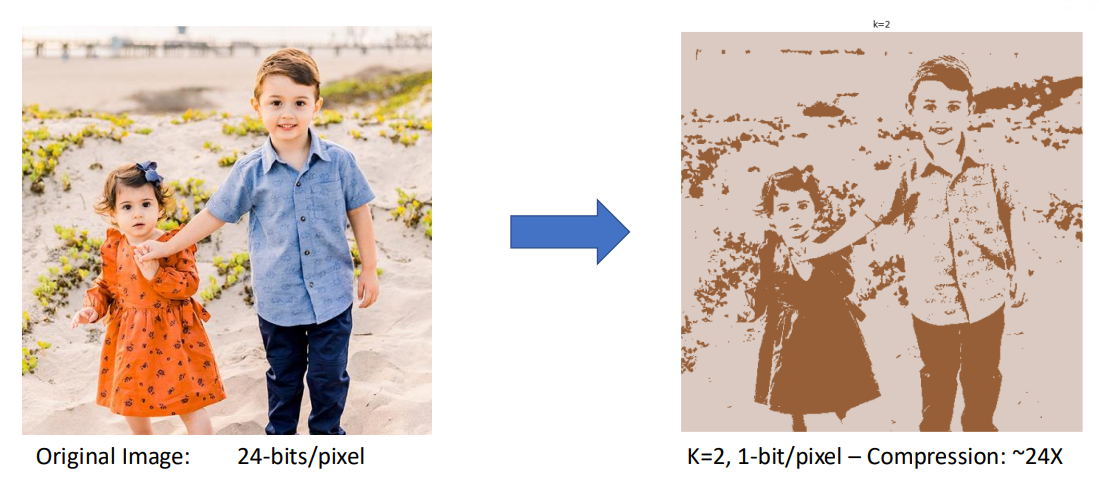
\includegraphics[width=0.4\textwidth]{../imgs/img-cluster-ex.png}
	\caption{K-Means: Image Compression}
\end{figure}

\subsection*{Issues with K-Means}
K-Means is a \textbf{non-convex} optimization problem, so the algorithm typically converges to a \textbf{local minimum}, not necessarily the global minimum. Consequently,
\begin{itemize}
	\item The same dataset may yield different clustering results under different initializations, and
	\item Initialization plays a critical role in the final outcome.
\end{itemize}

\begin{figure}[h]
	\centering
	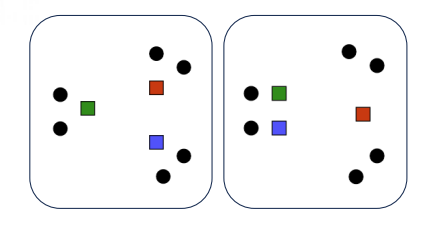
\includegraphics[width=0.35\textwidth]{../imgs/kissue.png}
	\caption{Different clusters on same input}
\end{figure}

\pagebreak

\subsection*{Choice of distance matters!}

\begin{figure}[h]
	\centering
	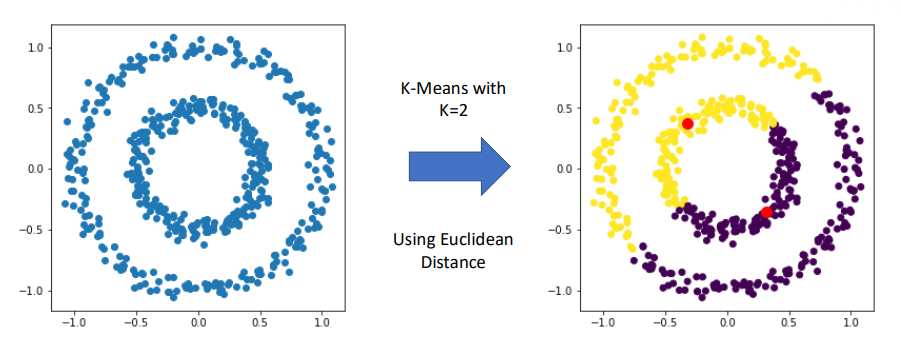
\includegraphics[width=0.35\textwidth]{../imgs/kmeans-euc.png}
	\caption{K-Means with euclidian distance}
\end{figure}

\begin{figure}[h]
	\centering
	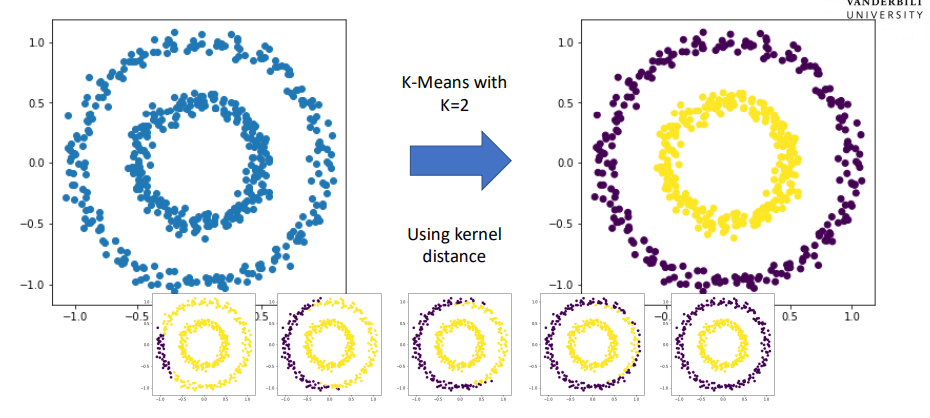
\includegraphics[width=0.35\textwidth]{../imgs/kmeans-ker.png}
	\caption{K-Means with kernel distance}
\end{figure}



\subsection*{How to find the right K}

\paragraph*{The Elbow Method}
Calculate the Within-Cluster-Sum of Squared Errors (WSS) for different values of k. In the plot of WSS versus-k, the optimal k value is visible as an elbow.

\paragraph*{The Silhouette Method}

\[
	s(o) = \frac{b(o) - a(o)}{\max\{a(o),\, b(o)\}}
\]

\noindent where:
\begin{itemize}
	\item $s(o)$ is the silhouette coefficient of data point $o$,
	\item $a(o)$ is the \textit{average distance} between $o$ and all other data points in the cluster to which $o$ belongs,
	\item $b(o)$ is the \textit{minimum average distance} from $o$ to all clusters to which $o$ does not belong.
\end{itemize}

The silhouette coefficient measures how well a data point fits within its assigned cluster and how far it is from neighboring clusters.

\[
	-1 \leq s(o) \leq 1
\]
\begin{itemize}
	\item $s(o) = 1$ indicates that the data point is well-clustered,
	\item $s(o) = -1$ indicates that the data point is misclassified,
	\item $s(o) = 0$ indicates that the data point lies on a cluster boundary.
\end{itemize}

We want to calculate $s(o)$ for different k values and choose the result with the highest score.

\pagebreak

\section*{Gaussian Mixture Models}
The idea here is to approximate with a mixture of Gaussian distributions.

Below is hte Gaussian (Normal) distrubtion formula, it tells us how likely (or typical) it is to observe a value near
$x$ given a Gaussian distribution with parameters $\mu$ and $\sigma$.
\[
	p(x; \mu, \sigma) = \mathcal{N}(x; \mu, \sigma) = \frac{1}{\sqrt{2\pi\sigma^2}} \, e^{ -\frac{(x - \mu)^2}{2\sigma^2} }
\]

We want to estimate the mean and standard deviation
from our observed samples $\{x_1, \dots, x_N\}$. We can do this using \textit{Maximum Likelihood Estimation (MLE)}.


\[
	\arg\max_{\mu, \sigma} \, p(x_1, \dots, x_N; \mu, \sigma) = \prod_{n=1}^{N} p(x_n; \mu, \sigma)
\]

Maximum Log-Likelihood

\[
	\arg\max_{\mu, \sigma} \log \left( \prod_{n=1}^{N} p(x_n; \mu, \sigma) \right) = \sum_{n=1}^{N} \log p(x_n; \mu, \sigma)
\]

Minimizing Negative Log-Likelihood

\[
	\arg\min_{\mu, \sigma} \sum_{n=1}^{N}
	\underbrace{
		\left[
			\frac{ \log(2\pi\sigma^2) }{2} + \frac{(x_n - \mu)^2}{2\sigma^2}
			\right]
	}_{L}
\]

\[
	\Rightarrow
	\begin{cases}
		\frac{\partial L}{\partial \mu} = 0 \Rightarrow \mu_* = \frac{1}{N} \sum_{n=1}^{N} x_n \\[1em]
		\frac{\partial L}{\partial \sigma} = 0 \Rightarrow \sigma^2_* = \frac{1}{N} \sum_{n=1}^{N} (x_n - \mu_*)^2
	\end{cases}
\]

We should notice these derived formulas are also just the empirical mean and variance formulas.

\paragraph*{2D data}
If our data is 2 dimensional we see the formulas as so:

\medskip

MLE:
\[
	p(x; \mu, \Sigma) = \frac{1}{\sqrt{(2\pi)^d \det(\Sigma)}}
	\exp\left( -\frac{1}{2} (x - \mu)^T \Sigma^{-1} (x - \mu) \right)
\]

Mean:
\[
	\frac{\partial L}{\partial \mu} = 0 \quad \Rightarrow \quad
	\mu_* = \frac{1}{N} \sum_{n=1}^{N} x_n
\]

Covariance:
\[
	\frac{\partial L}{\partial \Sigma} = 0 \quad \Rightarrow \quad
	\Sigma_* = \frac{1}{N} \sum_{n=1}^{N} (x_n - \mu_*)(x_n - \mu_*)^T
\]

\pagebreak

\paragraph*{Multiple Gaussians}

A Mixture of Gaussians (MoG) models the data as a weighted sum of $K$ Gaussian distributions:

\medskip
This formula telss us the overall probability density $p(x)$ of observing a data point $x$, assuming that the data is generated by a mixture (i.e., combination) of multiple Gaussian distributions.
\[
	p(x; \{(\alpha_k, \mu_k, \sigma_k)\}_{k=1}^K)
	= \sum_{k=1}^{K} \alpha_k \, \mathcal{N}(x; \mu_k, \sigma_k)
	= \sum_{k=1}^{K} \frac{\alpha_k}{\sqrt{2\pi\sigma_k^2}}
	\exp\left( -\frac{(x - \mu_k)^2}{2\sigma_k^2} \right)
\]

\textbf{Where:}
\begin{itemize}
	\item k is the number of gausians (clusters)
	\item $\alpha_k \geq 0$ are component weights
	\item $\sum_{k=1}^K \alpha_k = 1$
	\item $\sigma_k > 0$ (standard deviation of each Gaussian)
\end{itemize}

\paragraph*{Problem Setup}
Assume we have $N$ i.i.d. samples from a mixture of Gaussians:

\[
	\{x_n\}_{n=1}^N \sim p_d(x)
\]

We eant to estimate the parameters $\{(\alpha_k, \mu_k, \sigma_k)\}_{k=1}^K$ from the data.

\medskip

The likelihood of the full dataset is:

\[
	\prod_{n=1}^{N} \sum_{k=1}^{K} \alpha_k \, \mathcal{N}(x_n; \mu_k, \sigma_k)
\]

Taking the logarithm:

\[
	\log \left( \prod_{n=1}^{N} \sum_{k=1}^{K} \alpha_k \, \mathcal{N}(x_n; \mu_k, \sigma_k) \right)
	= \sum_{n=1}^{N} \log \left( \sum_{k=1}^{K} \alpha_k \, \mathcal{N}(x_n; \mu_k, \sigma_k) \right)
\]

The term $\log(\sum \cdot)$ is problematic for optimization!
This is where the \textbf{Expectation-Maximization (EM) algorithm} comes into play.

\subsection*{Expectation Maximization Algorithm}

If we knew which Gaussian component each data point came from (i.e., the component assignment), we could simply run MLE for each component separately.

\medskip

But we \textbf{don’t} observe which Gaussian generated each point. This assignment is treated as a \textbf{latent variable}.

\paragraph*{Latent Variable Definition}

Let:
$z = [z_1, z_2, \dots, z_K], \quad z_k \in \{0, 1\}$

Only one $z_k = 1$ (indicating which component generated $x$), the rest are 0. This is a one-hot vector.


\begin{itemize}
	\item Choose a component $k$ with probability $\alpha_k$
	      \[
		      p(z_k = 1) = \alpha_k
	      \]

	\item Then sample $x$ from the Gaussian associated with component $k$:
	      \[
		      p(x \mid z_k = 1) = \frac{1}{\sqrt{2\pi \sigma_k^2}} \exp\left(-\frac{(x - \mu_k)^2}{2\sigma_k^2}\right)
	      \]

	\item Total marginal likelihood of $x$ (mixture distribution):
	      \[
		      p(x) = \sum_{k=1}^{K} p(x \mid z_k = 1) \cdot p(z_k = 1)
		      = \sum_{k=1}^{K} \alpha_k \, \mathcal{N}(x; \mu_k, \sigma_k^2)
	      \]
\end{itemize}

\paragraph*{Posterior Assignment: E-Step}

We use Bayes’ rule to compute the \textbf{soft assignment} of data point $x$ to component $k$:

\[
	p(z_k = 1 \mid x) = \frac{p(x \mid z_k = 1) \cdot p(z_k = 1)}{p(x)}
	= \frac{ \alpha_k \, \mathcal{N}(x; \mu_k, \sigma_k^2) }{ \sum_{j=1}^K \alpha_j \, \mathcal{N}(x; \mu_j, \sigma_j^2) }
\]

This tells us the probability that a data point $x$ came from Gaussian $k$.

\bigskip

\noindent\textit{This completes the E-step of the EM algorithm.}

\paragraph*{Algorithm Process}

It alternates between:

\begin{itemize}
	\item \textbf{E-Step (Expectation):} Compute the probability that each data point belongs to each component (soft assignments).
	\item \textbf{M-Step (Maximization):} Update the parameters to maximize the expected log-likelihood based on the soft assignments.
\end{itemize}

\paragraph*{E-Step: Compute Responsibilities}

For fixed parameters $\{(\alpha_k, \mu_k, \sigma_k)\}_{k=1}^{K}$, compute the \textbf{responsibility} $r_n^k$ for each data point $x_n$ and each component $k$:

\[
	r_n^k = p(z_k = 1 \mid x_n)
	= \frac{ \alpha_k \, \mathcal{N}(x_n; \mu_k, \sigma_k^2) }
	{ \sum\limits_{i=1}^{K} \alpha_i \, \mathcal{N}(x_n; \mu_i, \sigma_i^2) }
\]

This is the posterior probability that data point $x_n$ was generated by component $k$.

\pagebreak

\paragraph*{M-Step: Update Parameters}

For fixed responsibilities $r_n^k$, update the parameters as follows:

\medskip

\textbf{1. Update Mixture Coefficients}

\[
	\alpha_k = \frac{N_k}{N}
	\; \; \text{for} \; \;
	N_k = \sum_{n=1}^{N} r_n^k
\]

\textbf{2. Update Means}

\[
	\mu_k = \frac{1}{N_k} \sum_{n=1}^{N} r_n^k x_n
\]

\textbf{3. Update Covariances}

\[
	\Sigma_k = \frac{1}{N_k} \sum_{n=1}^{N} r_n^k (x_n - \mu_k)(x_n - \mu_k)^T
\]

Repeat the E-step and M-step until the log-likelihood converges (or changes very little), or until a maximum number of iterations is reached.

\pagebreak

\subsection*{Example}
EM-GMM Algorithm (Input: x,k=2):

\begin{figure}[!ht]
	\centering

	\begin{subfigure}[t]{0.3\textwidth}
		\centering
		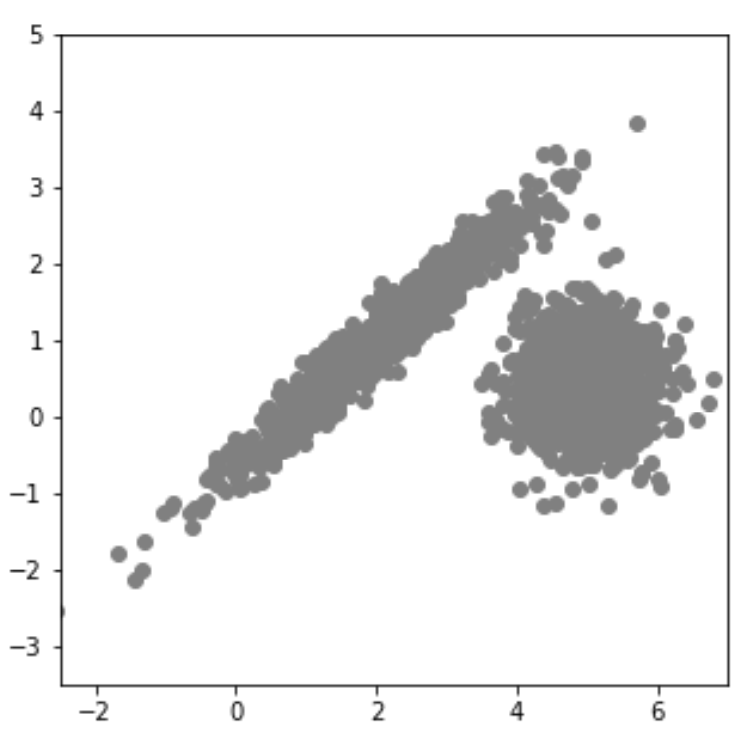
\includegraphics[width=\textwidth]{../imgs/gmm_p1.png}
		\caption*{\small Initialize means, variances, and weights randomly}
	\end{subfigure}
	\hspace{0.15\textwidth}
	\begin{subfigure}[t]{0.3\textwidth}
		\centering
		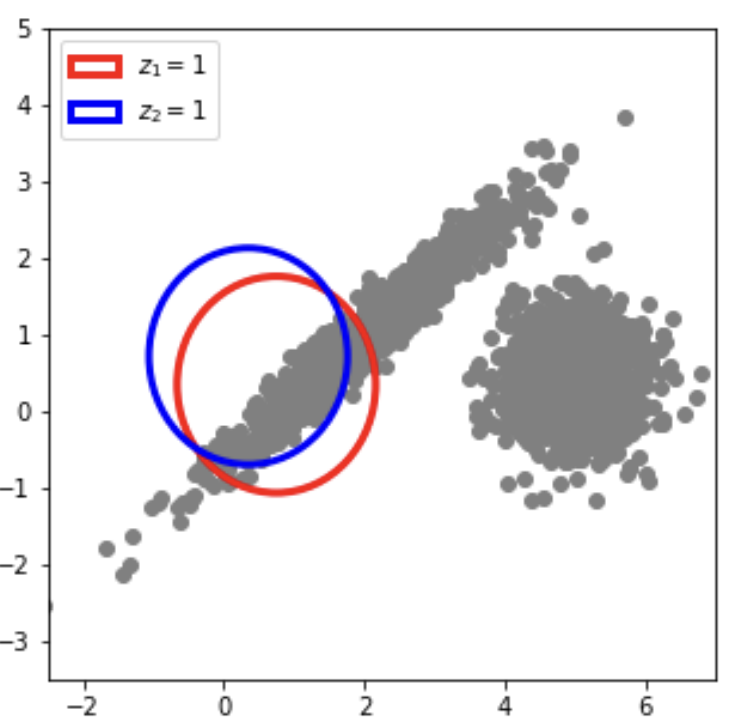
\includegraphics[width=\textwidth]{../imgs/gmm_p2.png}
		\caption*{\small E-step: compute responsibilities}
	\end{subfigure}

	\vspace{0.2em}

	\begin{subfigure}[t]{0.3\textwidth}
		\centering
		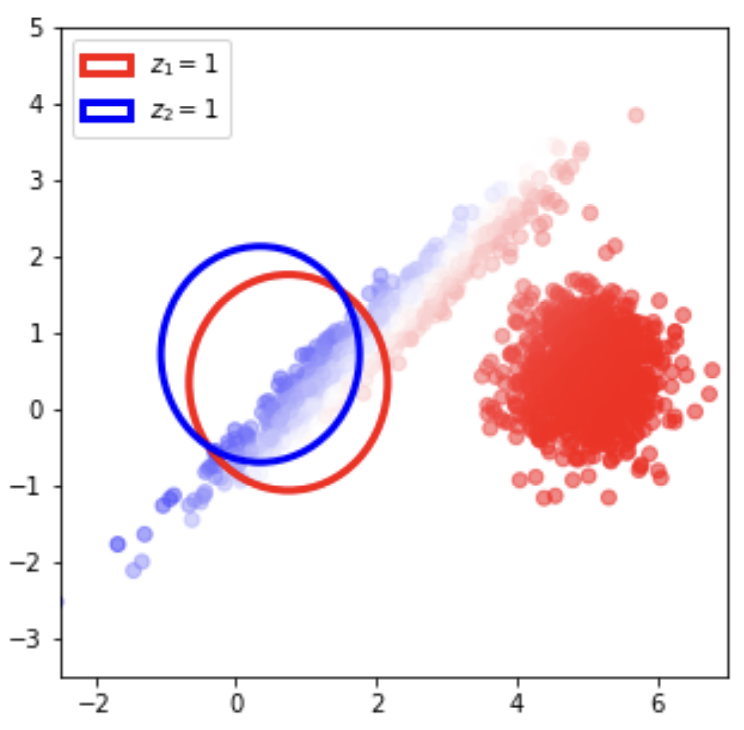
\includegraphics[width=\textwidth]{../imgs/gmm_p3.png}
		\caption*{\small M-step: update parameters}
	\end{subfigure}
	\hspace{0.15\textwidth}
	\begin{subfigure}[t]{0.3\textwidth}
		\centering
		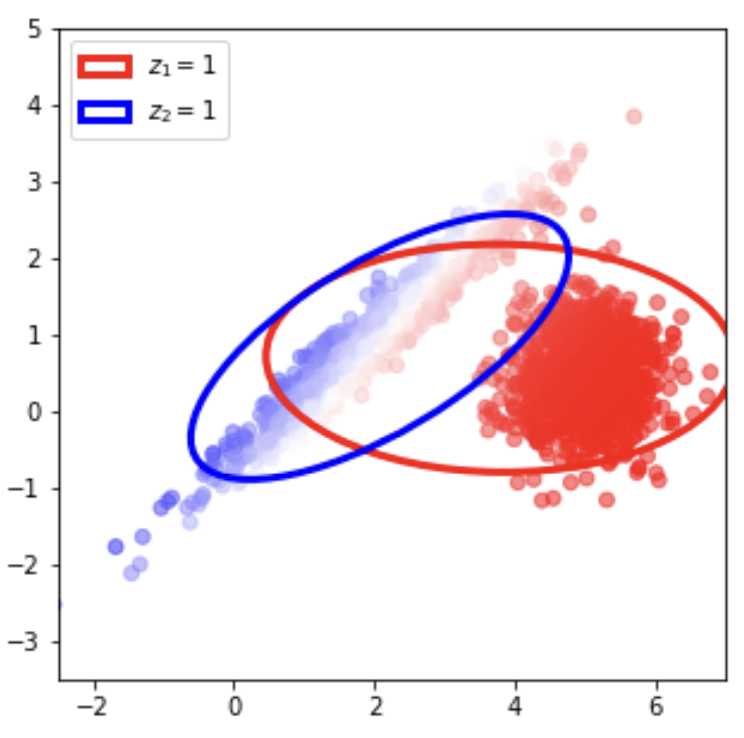
\includegraphics[width=\textwidth]{../imgs/gmm_p4.png}
		\caption*{\small Iterate E and M steps}
	\end{subfigure}

	\vspace{0.2em}

	\begin{subfigure}[t]{0.3\textwidth}
		\centering
		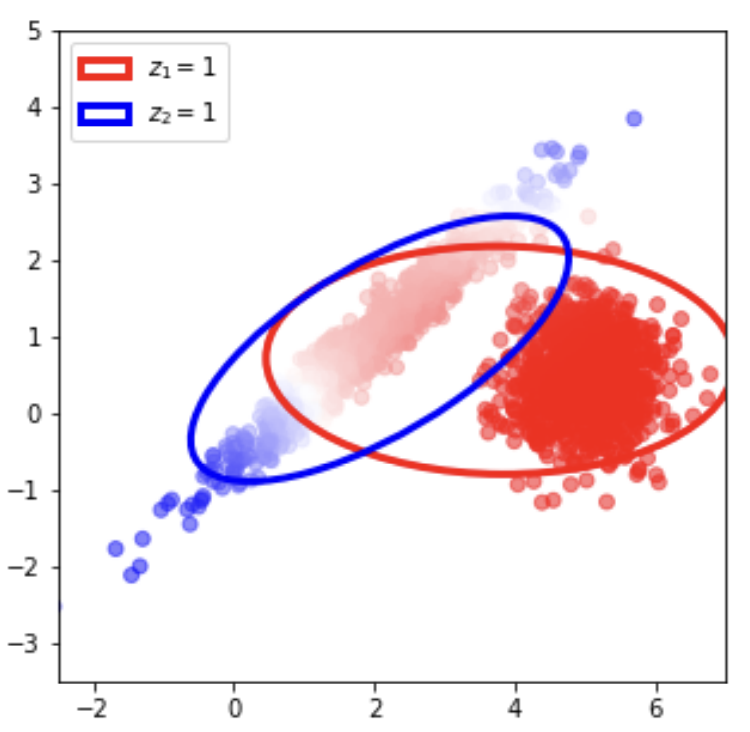
\includegraphics[width=\textwidth]{../imgs/gmm_p5.png}
		\caption*{\small Iterate E and M steps}
	\end{subfigure}
	\hspace{0.15\textwidth}
	\begin{subfigure}[t]{0.3\textwidth}
		\centering
		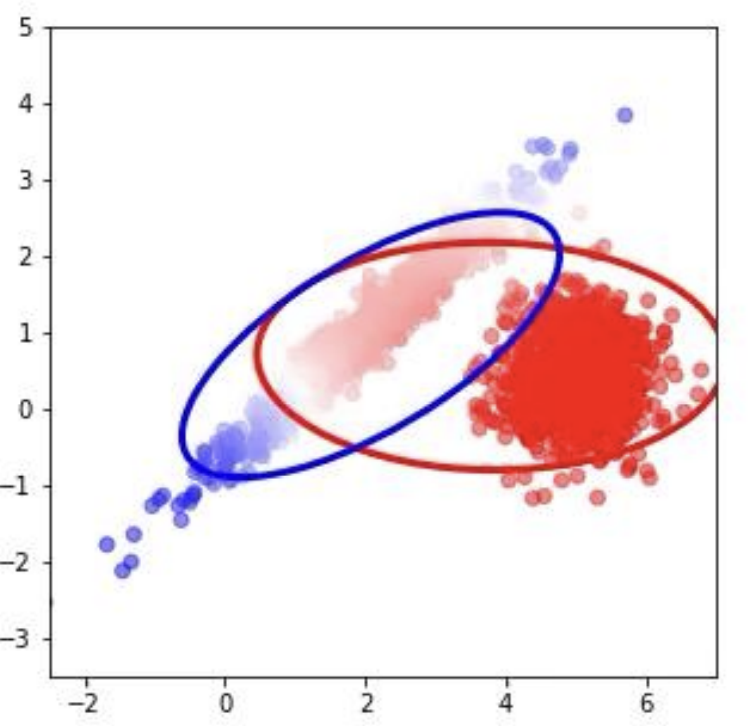
\includegraphics[width=\textwidth]{../imgs/gmm_p6.png}
    \caption*{\small Converged clusters}
	\end{subfigure}

	\caption{Visualization of the EM algorithm for GMM with $k = 2$ components}
\end{figure}




\section*{K-Means vs GMMs}

\begin{center}
	\begin{tabular}{|l|l|l|}
		\hline
		\textbf{Feature} & \textbf{K-Means}                                   & \textbf{GMMs}                   \\
		\hline
		Model type       & Geometric                                          & Probabilistic                   \\
		\hline
		Cluster shape    & Spherical                                          & Elliptical (full covariance)    \\
		\hline
		Assignment       & \textbf{Hard} (each point $\rightarrow$ 1 cluster) & \textbf{Soft} (probabilities)   \\
		\hline
		Objective        & Minimize squared distance                          & Maximize data likelihood        \\
		\hline
		Optimization     & Non-convex                                         & Non-convex                      \\
		\hline
		Output           & Cluster centers                                    & Means, covariances, and weights \\
		\hline
	\end{tabular}
\end{center}

\vspace{1em}

\noindent\textbf{K-means} can be seen as a \textit{special case} of a GMM where:
\begin{itemize}
	\item Covariances $\Sigma_k = \sigma^2 I$ are equal
	\item Only hard assignments are allowed
\end{itemize}

\end{document}



